% !Mode:: "TeX:UTF-8"
\documentclass{article}
\usepackage[UTF8,zihao=-4]{ctex}                     % 支持中文显示
\usepackage{graphicx}                       % 支持插图处理
% 支持版面尺寸设置
\usepackage{titlesec}                       % 控制标题的宏包
\usepackage{titletoc}                       % 控制目录的宏包
\usepackage{fancyhdr}                       % fancyhdr宏包 支持页眉和页脚的相关定义
\usepackage{color}                          % 支持彩色
\usepackage{amsmath}                        % AMSLaTeX宏包 用来排出更加漂亮的公式
\usepackage{amssymb}                        % 数学符号生成命令
\usepackage[below]{placeins}                %允许上一个section的浮动图形出现在下一个section的开始部分,还提供\FloatBarrier命令,使所有未处理的浮动图形立即被处理
\usepackage{flafter}                        % 使得所有浮动体不能被放置在其浮动环境之前,以免浮动体在引述它的文本之前出现.
\usepackage{multirow}                       % 使用Multirow宏包,使得表格可以合并多个row格
\usepackage{booktabs}                       % 表格,横的粗线;\specialrule{1pt}{0pt}{0pt}
\usepackage{longtable}                      % 支持跨页的表格。
\usepackage{tabularx}                       % 自动设置表格的列宽
\usepackage{subfigure}                      % 支持子图 %centerlast 设置最后一行是否居中
\usepackage[subfigure]{ccaption}            % 支持子图的中文标题
\usepackage[sort&compress,numbers]{natbib}  % 支持引用缩写的宏包
\usepackage{enumitem}                       % 使用enumitem宏包,改变列表项的格式
\usepackage{calc}                           % 长度可以用+ - * / 进行计算
\usepackage{txfonts}                        % 字体宏包
\usepackage{bm}                             % 处理数学公式中的黑斜体的宏包
\usepackage[amsmath,thmmarks,hyperref]{ntheorem}  % 定理类环境宏包,其中 amsmath 选项用来兼容 AMS LaTeX 的宏包
%如果您的pdf制作中文书签有乱码使用如下命令,就可以解决了
\usepackage{hyperref}
%%%%%%%%%%%%%%算法环境%%%%%%%%%%%%%%
\usepackage{listings}
\usepackage{xcolor}
\definecolor{dkgreen}{rgb}{0,0.6,0}
\definecolor{gray}{rgb}{0.5,0.5,0.5}
\definecolor{mauve}{rgb}{0.58,0,0.82}
\lstset{
	backgroundcolor=\color{gray!5},
	basicstyle={\linespread{1.1}\footnotesize\ttfamily},
	breakatwhitespace=true,
	breaklines=true,
	commentstyle=\color{dkgreen},
	frame=single,
	frameshape={RYRYNYYYY}{yny}{yny}{RYRYNYYYY},
	keywordstyle=\color{blue},
	language=Python,
	numbers=none,
	numberstyle=\tiny\color{gray},
	rulecolor=\color{gray!35},
	showstringspaces=false,
	stringstyle=\color{mauve},
	tabsize=4,
	aboveskip=3mm,
	belowskip=3mm,
	columns=flexible,
	framerule=1pt,
}
%%%%%%%%%%%%%%算法环境%%%%%%%%%%%%%%
%%%%%%%%%%%%去除目录红框%%%%%%%%%%%%
\hypersetup{
	colorlinks=true,
	linkcolor=black,
}
%%%%%%%%%%%%去除目录红框%%%%%%%%%%%%
%%%%%%%%%%%%%调整页边距%%%%%%%%%%%%%
\usepackage{geometry}
\geometry{a4paper,left=2cm,right=2cm,top=2cm,bottom=2cm}
%%%%%%%%%%%%%调整页边距%%%%%%%%%%%%%
\usepackage{appendix}
\usepackage{float}









\begin{document}

\title{图像处理第四次作业}
\author{刘坤鑫\thanks{3017218061 软件工程一班}}
\date{\today}
\maketitle
\begin{abstract}
本文主要实现了Shape Context算法,并对结果进行了分析。
\end{abstract}

\section{Shape Context}

\subsection{原理}

根据维基百科\footnote{\url{https://en.wikipedia.org/wiki/Shape_context}}及原始论文\footnote{\url{https://ieeexplore.ieee.org/stamp/stamp.jsp?arnumber=853834}},形状上下文算法可描述如下:

\begin{enumerate}
	\item Finding a list of points on shape edges. 将图像边缘提取出来,并对边缘进行均匀采样。
\begin{figure}[ht]
	\centering
	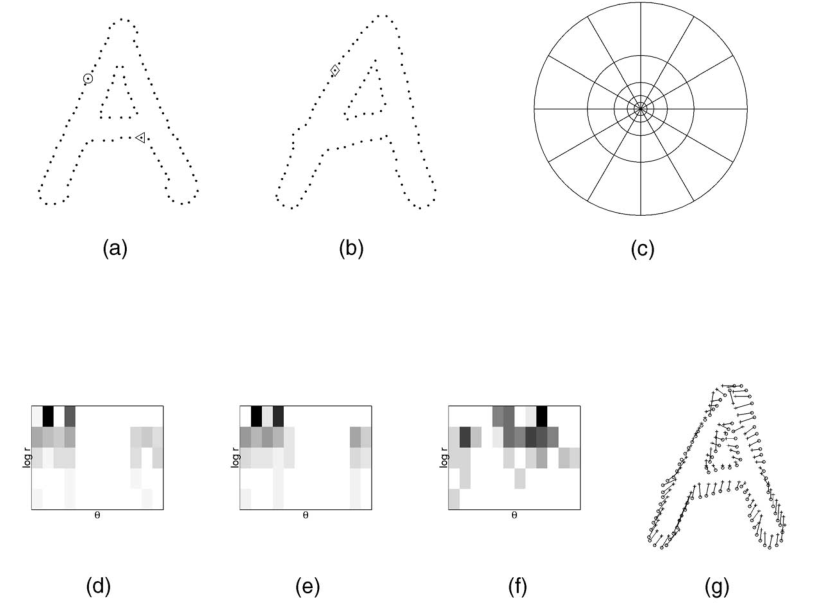
\includegraphics[width=0.7\linewidth]{fig/1}
	\caption{k-bin统计图}
	\label{fig:1}
\end{figure}
	\item Computing the shape context. 如图\ref{fig:1}所示,计算形状上下文,即论文中的k-bin图。计算方法如下:对采样的每个点,统计出其他所有点到其的方位角及对数距离的值。
	\item Computing the cost matrix. 计算费用矩阵。费用矩阵中,行表示图A的所有采样点,列表示图B的所有采样点,采样点的费用计算根据统计图得到。计算公式如下:
\begin{equation}
C_{S}=\frac{1}{2} \sum_{k=1}^{K} \frac{[g(k)-h(k)]^{2}}{g(k)+h(k)}
\end{equation}
	\item Finding the matching that minimizes total cost. 给两个图的采样点进行一一对应匹配,使得总费用最小。问题转化为经典的带权二分图匹配,可用改进的匈牙利算法KM算法求出,时间复杂度为$O(n^3)$
\end{enumerate}

\section{详细设计}

见附录(内含注释)。

\section{结果及结论}

如图所示\ref{fig:2},第一张为原图字母A,后面为处理后的图像及对照字母D。

如图所示\ref{fig:3},为提取边缘后的图像。

如图所示\ref{fig:4},均匀采样200个点后的图像。

\begin{figure}[H]
	\centering
	\subfigure[A0.png]{
		
\includegraphics[width=3.2cm]{../code/pic/A0.png}
	}
	\quad
	\subfigure[A1.png]{
		
\includegraphics[width=3.2cm]{../code/pic/A1.png}
	}
	\quad
	\subfigure[A2.png]{
		
\includegraphics[width=3.2cm]{../code/pic/A2.png}
	}
	\\
	\subfigure[A3.png]{
		
\includegraphics[width=3.2cm]{../code/pic/A3.png}
	}
	\quad
	\subfigure[A4.png]{
		
\includegraphics[width=3.2cm]{../code/pic/A4.png}
	}
	\quad
	\subfigure[A5.png]{
		
\includegraphics[width=3.2cm]{../code/pic/A5.png}
	}
	\caption{原始图像}
	\label{fig:2}
\end{figure}

\begin{figure}[H]
	\centering
	\subfigure[A\_points0.png]{
		
\includegraphics[width=3.2cm]{../code/pic/A_points0.png}
	}
	\quad
	\subfigure[A\_points1.png]{
		
\includegraphics[width=3.2cm]{../code/pic/A_points1.png}
	}
	\quad
	\subfigure[A\_points2.png]{
		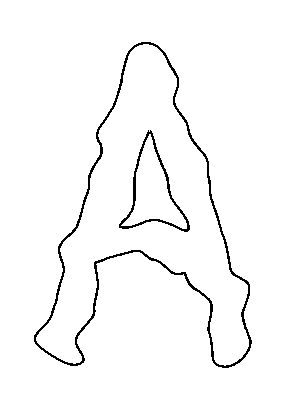
\includegraphics[width=3.2cm]{../code/pic/A_points2.png}
	}
	\\
	\subfigure[A\_points3.png]{
		
\includegraphics[width=3.2cm]{../code/pic/A_points3.png}
	}
	\quad
	\subfigure[A\_points4.png]{
		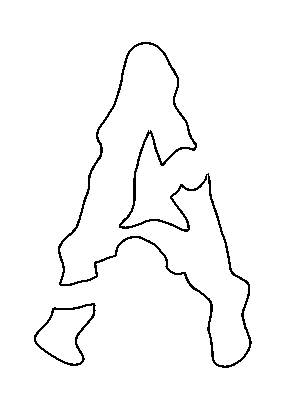
\includegraphics[width=3.2cm]{../code/pic/A_points4.png}
	}
	\quad
	\subfigure[A\_points5.png]{
		
\includegraphics[width=3.2cm]{../code/pic/A_points5.png}
	}
	\caption{提取边缘后的图像}
	\label{fig:3}
\end{figure}

\begin{figure}[H]
	\centering
	\subfigure[A\_points\_sample0.png]{
		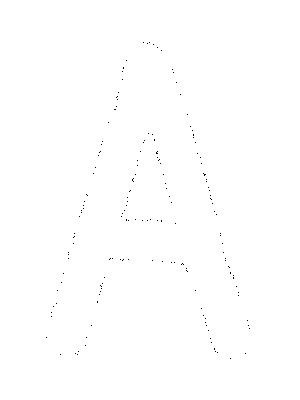
\includegraphics[width=3.2cm]{../code/pic/A_points_sample0.png}
	}
	\quad
	\subfigure[A\_points\_sample1.png]{
		
\includegraphics[width=3.2cm]{../code/pic/A_points_sample1.png}
	}
	\quad
	\subfigure[A\_points\_sample2.png]{
		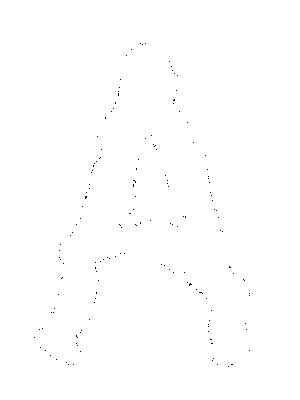
\includegraphics[width=3.2cm]{../code/pic/A_points_sample2.png}
	}
	\\
	\subfigure[A\_points\_sample3.png]{
		
\includegraphics[width=3.2cm]{../code/pic/A_points_sample3.png}
	}
	\quad
	\subfigure[A\_points\_sample4.png]{
		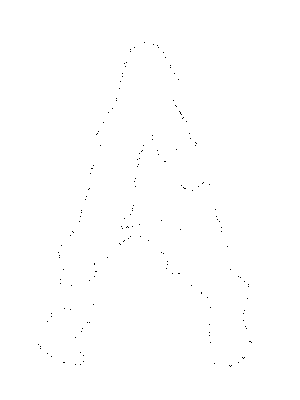
\includegraphics[width=3.2cm]{../code/pic/A_points_sample4.png}
	}
	\quad
	\subfigure[A\_points\_sample5.png]{
		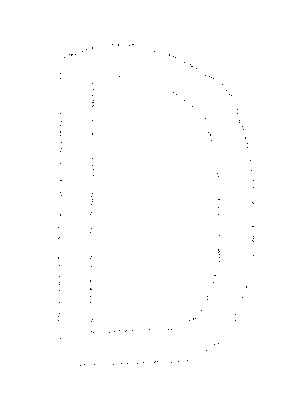
\includegraphics[width=3.2cm]{../code/pic/A_points_sample5.png}
	}
	\caption{均匀采样200个点后的图像}
	\label{fig:4}
\end{figure}

如表\ref{tbl:1}所示为不同采样点数的计算结果,如表\ref{tbl:2}所示为原图与其他图像的结果。可以看出,原图经过平移、缩放、略微变形等处理后,计算结果几乎无变化。如果形状变化过大,结果就会变大。如果采样点数越多,精确程度越高,当然运行时间越慢。

\begin{table}[ht]
	\label{tbl:1}
	\centering
	\caption{不同采样点数的计算结果}
	\begin{tabular}{|c|c|}
		\hline

		采样点数 & 结果 \\ \hline
		50 & 2053 \\ \hline
		100 & 8020 \\ \hline
		200 & 32142 \\ \hline
		
	\end{tabular}
\end{table}

\begin{table}[ht]
	\label{tbl:2}
	\centering
	\caption{原图与其他图像的结果}
	\begin{tabular}{|c|c|}
		\hline
		
		图像编号(原图为0) & 结果 \\ \hline
		1 & 8020 \\ \hline
		2 & 8091 \\ \hline
		3 & 8104 \\ \hline
		4 & 7990 \\ \hline
		5 & 8326 \\ \hline
		
	\end{tabular}
\end{table}









\clearpage
\begin{appendix}
	\section{完整源码}
	

	\lstinputlisting[title={ShapeContext.py}]{../code/ShapeContext.py}
	
	
\end{appendix}





























\end{document}

